%%%%%%%%%%%%%%%%%%%%%%%%%%%%%%%%%%%%%%%%%%%%%%%%%%%%%%%%%%%%%%%%%%%%%%%%%%%%%%%%%
%%%%%                           ONLINE APPENDIX                              %%%%
%%%%%%%%%%%%%%%%%%%%%%%%%%%%%%%%%%%%%%%%%%%%%%%%%%%%%%%%%%%%%%%%%%%%%%%%%%%%%%%%%

%%%%%%%%%%%%%%%%%%%%%%%%%%%%%%%%%%%%%%%%%%%%%%%%%%%%%%%%%%%%%%%%%%%%%%%%%%%%%%%%%
\section{Appendix Tables}

\begin{table}[h!]
	\caption{Dynamic DiD: cumulative effect over 6 months}
	\label{tab:dynamic_cumulative}
	\centering
	\resizebox{0.7\textwidth}{!}{
		\vspace{0pt}    
		{
\def\sym#1{\ifmmode^{#1}\else\(^{#1}\)\fi}
\begin{tabular}{l*{5}{c}}
\hline\hline
          &\multicolumn{1}{c}{(1)}         &\multicolumn{1}{c}{(2)}         &\multicolumn{1}{c}{(3)}         &\multicolumn{1}{c}{(4)}         &\multicolumn{1}{c}{(5)}         \\
\hline
Sum of MW effects&   0.0566         &   0.0554         &   0.0562         &   0.0563         &   0.0556         \\
          & (0.0347)         & (0.0345)         & (0.0343)         & (0.0343)         & (0.0342)         \\
\hline
Wage controls&       No         &      Yes         &      Yes         &       No         &      Yes         \\
Employment controls&       No         &       No         &       No         &       No         &      Yes         \\
Establishment-count controls&       No         &       No         &       No         &      Yes         &      Yes         \\
Observations&  106,446         &  104,360         &  104,360         &  106,160         &  104,360         \\
\hline\hline
\end{tabular}
}

	}
	\begin{minipage}{.95\textwidth} \footnotesize
		\vspace{3mm} 
		\textit{Notes}: The table shows estimates for the cumulative impact of MW (log) changes 
		on (log) rents changes over 6 months. Coefficients are obtained by taking the sum of 
		$\hat{\beta}_{r}$, estimated via \autoref{eq:lags}: $\sum\limits_{r=0}^{5} \hat{\beta}_{r}$. 
		Standard errors clustered at the state level. *** $p < 0.01$, ** $p < 0.05$, * $p < 0.1$.   
	\end{minipage}
\end{table}

\clearpage
\begin{landscape}
	\begin{table}[h!]
	    \caption{Results from different dynamic models}
	    \label{tab:horse_race_main}
	    \centering
	    \resizebox{1.2\textwidth}{!}{
		    \vspace{0pt}    
		    {
\def\sym#1{\ifmmode^{#1}\else\(^{#1}\)\fi}
\begin{tabular}{l*{5}{c}}
\hline\hline
          &\multicolumn{1}{c}{(1)}&\multicolumn{1}{c}{(2)}&\multicolumn{1}{c}{(3)}&\multicolumn{1}{c}{(4)}&\multicolumn{1}{c}{(5)}\\
          &\multicolumn{1}{c}{DiD}&\multicolumn{1}{c}{Distributed leads and lags}&\multicolumn{1}{c}{Distributed Lags}&\multicolumn{1}{c}{AB distributed leads and lags}&\multicolumn{1}{c}{AB distributed lags}\\
\hline
\Delta ln(MW)\_{t-3}&                  & 0.000493         &                  & 0.000164         &                  \\
          &                  &(0.00833)         &                  &(0.00889)         &                  \\
[1em]
\Delta ln(MW)\_{t-2}&                  &  0.00520         &                  &  0.00527         &                  \\
          &                  & (0.0122)         &                  & (0.0112)         &                  \\
[1em]
\Delta ln(MW)\_{t-1}&                  & -0.00115         &                  & -0.00262         &                  \\
          &                  & (0.0130)         &                  & (0.0107)         &                  \\
[1em]
\Delta ln(MW)\_{t}&   0.0256\sym{**} &   0.0267\sym{**} &   0.0261\sym{**} &   0.0265\sym{**} &   0.0261\sym{**} \\
          & (0.0121)         & (0.0123)         & (0.0126)         & (0.0107)         & (0.0109)         \\
[1em]
\Delta ln(MW)\_{t+1}&                  &   0.0161\sym{*}  &   0.0158\sym{*}  &   0.0225\sym{**} &   0.0223\sym{**} \\
          &                  &(0.00833)         &(0.00812)         &(0.00943)         &(0.00938)         \\
[1em]
\Delta ln(MW)\_{t+2}&                  & -0.00758         & -0.00714         & -0.00381         & -0.00331         \\
          &                  & (0.0126)         & (0.0128)         & (0.0132)         & (0.0134)         \\
[1em]
\Delta ln(MW)\_{t+3}&                  &  0.00280         &  0.00342         &  0.00117         &  0.00195         \\
          &                  &(0.00832)         &(0.00819)         &(0.00983)         &(0.00978)         \\
[1em]
\Delta ln(y)\_{t-1}&                  &                  &                  &   -0.241\sym{***}&   -0.239\sym{***}\\
          &                  &                  &                  &(0.00633)         &(0.00618)         \\
\hline
R-squared &    0.024         &    0.024         &    0.024         &    0.081         &    0.080         \\
Observations&   112232         &   108780         &   112209         &   107654         &   111083         \\
\hline\hline
\end{tabular}
}

	    }
	    \begin{minipage}{1.15\textwidth} \footnotesize
			\vspace{3mm} 
			\textit{Notes}: The table presents baseline estimates obtained from \autoref{eq:did}, 
			(\ref{eq:leads_lags}), and (\ref{eq:lags}) in columns (1), (2), and (3) respectively. 
			Column (4) allows for rental price dynamics by adding the lagged change in (log) rents, 
			$\Delta y_{i(t-1)}$, and it is estimated instrumenting it with a deeper lag $\Delta 
			y_{i(t-2)}$ \parencite{arellano1991some}. Similarly, column (5) solves for 
			\autoref{eq:ab_panel} where only lags of MW changes are allowed. Finally, columns (6) and 
			(7) instrument $\Delta y_{i(t-1)}$ with an off-window lag of the MW (log) change, $\Delta 
			\title{MW}_{i(t-6)}$ for the leads and lags, and lags only versions of the model. All 
			specifications additionally control for a zipcode-level linear trend. Standard errors 
			clustered at the state level. *** $p < 0.01$, ** $p < 0.05$, * $p < 0.1$.   
		\end{minipage}
	\end{table}
\end{landscape}

\clearpage
\begin{table}[h!]
    \caption{Comparison between unbalanced and baseline panel model estimation}
    \label{tab:comparison_unbal_base}
    \centering
     \resizebox{\textwidth}{!}{
    \vspace{0pt}    
    {
\def\sym#1{\ifmmode^{#1}\else\(^{#1}\)\fi}
\begin{tabular}{l*{6}{c}}
\hline\hline
          &\multicolumn{3}{c}{Unbalanced Panel}                    &\multicolumn{3}{c}{Baseline Panel}                      \\\cmidrule(lr){2-4}\cmidrule(lr){5-7}
          &\multicolumn{1}{c}{(1)}&\multicolumn{1}{c}{(2)}&\multicolumn{1}{c}{(3)}&\multicolumn{1}{c}{(4)}&\multicolumn{1}{c}{(5)}&\multicolumn{1}{c}{(6)}\\
          &\multicolumn{1}{c}{DiD}&\multicolumn{1}{c}{\shortstack{Distributed \\ leads and lags}}&\multicolumn{1}{c}{\shortstack{Distributed \\ Lags}}&\multicolumn{1}{c}{DiD}&\multicolumn{1}{c}{\shortstack{Distributed \\ leads and lags}}&\multicolumn{1}{c}{\shortstack{Distributed \\ Lags}}\\
\hline
$\Delta \ln(MW)_{t-5}$&                  &  -0.0115         &                  &                  &  -0.0153         &                  \\
          &                  &(0.00810)         &                  &                  &(0.00915)         &                  \\
[1em]
$\Delta \ln(MW)_{t-4}$&                  & -0.00812         &                  &                  & -0.00306         &                  \\
          &                  &(0.00792)         &                  &                  & (0.0110)         &                  \\
[1em]
$\Delta \ln(MW)_{t-3}$&                  & -0.00171         &                  &                  & 0.000380         &                  \\
          &                  &(0.00864)         &                  &                  &(0.00829)         &                  \\
[1em]
$\Delta \ln(MW)_{t-2}$&                  & -0.00233         &                  &                  &  0.00531         &                  \\
          &                  &(0.00743)         &                  &                  & (0.0121)         &                  \\
[1em]
$\Delta \ln(MW)_{t-1}$&                  &  0.00552         &                  &                  &-0.000798         &                  \\
          &                  &(0.00823)         &                  &                  & (0.0126)         &                  \\
[1em]
$\Delta \ln(MW)_{t}$&   0.0220\sym{*}  &   0.0218\sym{*}  &   0.0229\sym{*}  &   0.0257\sym{**} &   0.0265\sym{**} &   0.0268\sym{**} \\
          & (0.0111)         & (0.0117)         & (0.0115)         & (0.0120)         & (0.0119)         & (0.0126)         \\
[1em]
$\Delta \ln(MW)_{t+1}$&                  &  0.00473         &  0.00788         &                  &   0.0128\sym{*}  &   0.0162\sym{*}  \\
          &                  &(0.00574)         &(0.00586)         &                  &(0.00739)         &(0.00816)         \\
[1em]
$\Delta \ln(MW)_{t+2}$&                  &  0.00405         &  0.00558         &                  & -0.00785         & -0.00623         \\
          &                  &(0.00915)         &(0.00772)         &                  & (0.0135)         & (0.0128)         \\
[1em]
$\Delta \ln(MW)_{t+3}$&                  &  0.00347         &  0.00638         &                  &  0.00277         &  0.00359         \\
          &                  &(0.00632)         &(0.00636)         &                  &(0.00751)         &(0.00830)         \\
[1em]
$\Delta \ln(MW)_{t+4}$&                  &  0.00515         &  0.00505         &                  &  0.00994         &   0.0108         \\
          &                  &(0.00688)         &(0.00684)         &                  &(0.00695)         &(0.00704)         \\
[1em]
$\Delta \ln(MW)_{t+5}$&                  & 0.000767         & -0.00261         &                  &  0.00778         &  0.00641         \\
          &                  &(0.00774)         &(0.00800)         &                  &(0.00735)         &(0.00691)         \\
\hline
Observations&   194295         &   177659         &   194209         &   112232         &   106446         &   112161         \\
\hline\hline
\end{tabular}
}

    }
    \begin{minipage}{.95\textwidth} \footnotesize
		\vspace{3mm} 
		\textit{Notes}: The table compares estimates from our main specifications (\textit{static DiD}, 
		\textit{distributed leads and lags DiD}, and \textit{distributed lags DiD}) obtained using the 
		baseline sample with estimates obtained using the unbalanced, full sample of zipcodes. Columns 
		(1), (2), and (3) show results from from \autoref{eq:did}, (\ref{eq:leads_lags}), and (\ref{eq:lags}) 
		respectively, using the unbalanced sample. All three columns additionally control for ``cohort 
		$\times$ period" FE to account for differences in the each zipcodes time series. Columns (4), (5), 
		and (6) replicates our main results obtained with the baseline sample and presented in 
		\autoref{tab: did_main}, column (2), \autoref{tab: dynamic_lags_leads_main}, column (2) and 
		\autoref{tab:horse_race_main}. All specifications control for zipcode-level linear trends. 
		Standard errors clustered at the state level. *** $p < 0.01$, ** $p < 0.05$, * $p < 0.1$.  
	\end{minipage}
\end{table}

\clearpage
\begin{table}[h!]
    \caption{Comparison between baseline and re-weighted panel model estimation}
    \label{tab:comparison_wgt_base}
    \centering
    \resizebox{\textwidth}{!}{
	    \vspace{0pt}    
	    {
\def\sym#1{\ifmmode^{#1}\else\(^{#1}\)\fi}
\begin{tabular}{l*{6}{c}}
\hline\hline
          &\multicolumn{3}{c}{Reweighted Panel}                    &\multicolumn{3}{c}{Baseline Panel}                      \\\cmidrule(lr){2-4}\cmidrule(lr){5-7}
          &\multicolumn{1}{c}{(1)}&\multicolumn{1}{c}{(2)}&\multicolumn{1}{c}{(3)}&\multicolumn{1}{c}{(4)}&\multicolumn{1}{c}{(5)}&\multicolumn{1}{c}{(6)}\\
          &\multicolumn{1}{c}{DiD}&\multicolumn{1}{c}{\shortstack{Distributed \\ leads and lags}}&\multicolumn{1}{c}{\shortstack{Distributed \\ Lags}}&\multicolumn{1}{c}{DiD}&\multicolumn{1}{c}{\shortstack{Distributed \\ leads and lags}}&\multicolumn{1}{c}{\shortstack{Distributed \\ Lags}}\\
\hline
$\Delta \ln(MW)_{t-5}$&                  & -0.00832         &                  &                  &  -0.0153         &                  \\
          &                  &(0.00687)         &                  &                  &(0.00915)         &                  \\
[1em]
$\Delta \ln(MW)_{t-4}$&                  &  0.00566         &                  &                  & -0.00306         &                  \\
          &                  &(0.00726)         &                  &                  & (0.0110)         &                  \\
[1em]
$\Delta \ln(MW)_{t-3}$&                  &  0.00821         &                  &                  & 0.000380         &                  \\
          &                  &(0.00905)         &                  &                  &(0.00829)         &                  \\
[1em]
$\Delta \ln(MW)_{t-2}$&                  &-0.000403         &                  &                  &  0.00531         &                  \\
          &                  & (0.0115)         &                  &                  & (0.0121)         &                  \\
[1em]
$\Delta \ln(MW)_{t-1}$&                  & -0.00860         &                  &                  &-0.000798         &                  \\
          &                  & (0.0116)         &                  &                  & (0.0126)         &                  \\
[1em]
$\Delta \ln(MW)_{t}$&   0.0365\sym{***}&   0.0369\sym{***}&   0.0372\sym{***}&   0.0257\sym{**} &   0.0265\sym{**} &   0.0268\sym{**} \\
          & (0.0124)         & (0.0127)         & (0.0132)         & (0.0120)         & (0.0119)         & (0.0126)         \\
[1em]
$\Delta \ln(MW)_{t+1}$&                  &  0.00782         &  0.00942         &                  &   0.0128\sym{*}  &   0.0162\sym{*}  \\
          &                  &(0.00706)         &(0.00730)         &                  &(0.00739)         &(0.00816)         \\
[1em]
$\Delta \ln(MW)_{t+2}$&                  & -0.00822         & -0.00694         &                  & -0.00785         & -0.00623         \\
          &                  & (0.0167)         & (0.0160)         &                  & (0.0135)         & (0.0128)         \\
[1em]
$\Delta \ln(MW)_{t+3}$&                  &  0.00560         &  0.00516         &                  &  0.00277         &  0.00359         \\
          &                  &(0.00600)         &(0.00693)         &                  &(0.00751)         &(0.00830)         \\
[1em]
$\Delta \ln(MW)_{t+4}$&                  &   0.0100         &   0.0103         &                  &  0.00994         &   0.0108         \\
          &                  &(0.00939)         &(0.00935)         &                  &(0.00695)         &(0.00704)         \\
[1em]
$\Delta \ln(MW)_{t+5}$&                  &  0.00798         &  0.00781         &                  &  0.00778         &  0.00641         \\
          &                  &(0.00808)         &(0.00870)         &                  &(0.00735)         &(0.00691)         \\
\hline
Observations&  112,232         &  106,446         &  112,161         &  112,232         &  106,446         &  112,161         \\
\hline\hline
\end{tabular}
}

    }
    \begin{minipage}{.95\textwidth} \footnotesize
		\vspace{3mm} 
		\textit{Notes}: The table compares estimates from our main specifications (\textit{static 
		DiD}, \textit{distributed leads and lags DiD}, and \textit{distributed lags DiD}) obtained 
		using the baseline sample with estimates obtained using the reweighted sample (see 
		\autoref{sec:sample_rest} for more details on how the weights are built). Columns (1), (2), 
		and (3) show results from from \autoref{eq:did}, (\ref{eq:leads_lags}), and (\ref{eq:lags}) 
		respectively, using the unbalanced sample. All three columns additionally control for 
		``cohort $\times$ period" FE to account for differences in the each zipcodes time series. 
		Columns (4), (5), and (6) replicates our main results obtained with the baseline sample 
		and presented in \autoref{tab: did_main}, column (2), \autoref{tab: dynamic_lags_leads_main}, 
		column (2) and \autoref{tab:horse_race_main}. All specifications control for zipcode-level 
		linear trends. Standard errors clustered at the state level. *** $p < 0.01$, ** $p < 0.05$, 
		* $p < 0.1$.
	\end{minipage}
\end{table}

\clearpage
%%%%%%%%%%%%%%%%%%%%%%%%%%%%%%%%%%%%%%%%%%%%%%%%%%%%%%%%%%%%%%%%%%%%%%%%%%%%%%%%%
\section{Appendix Figures}

\begin{figure}[!h]
	\caption{Dynamic DiD model comparison - local shocks}
	\label{fig:}
	\centering
	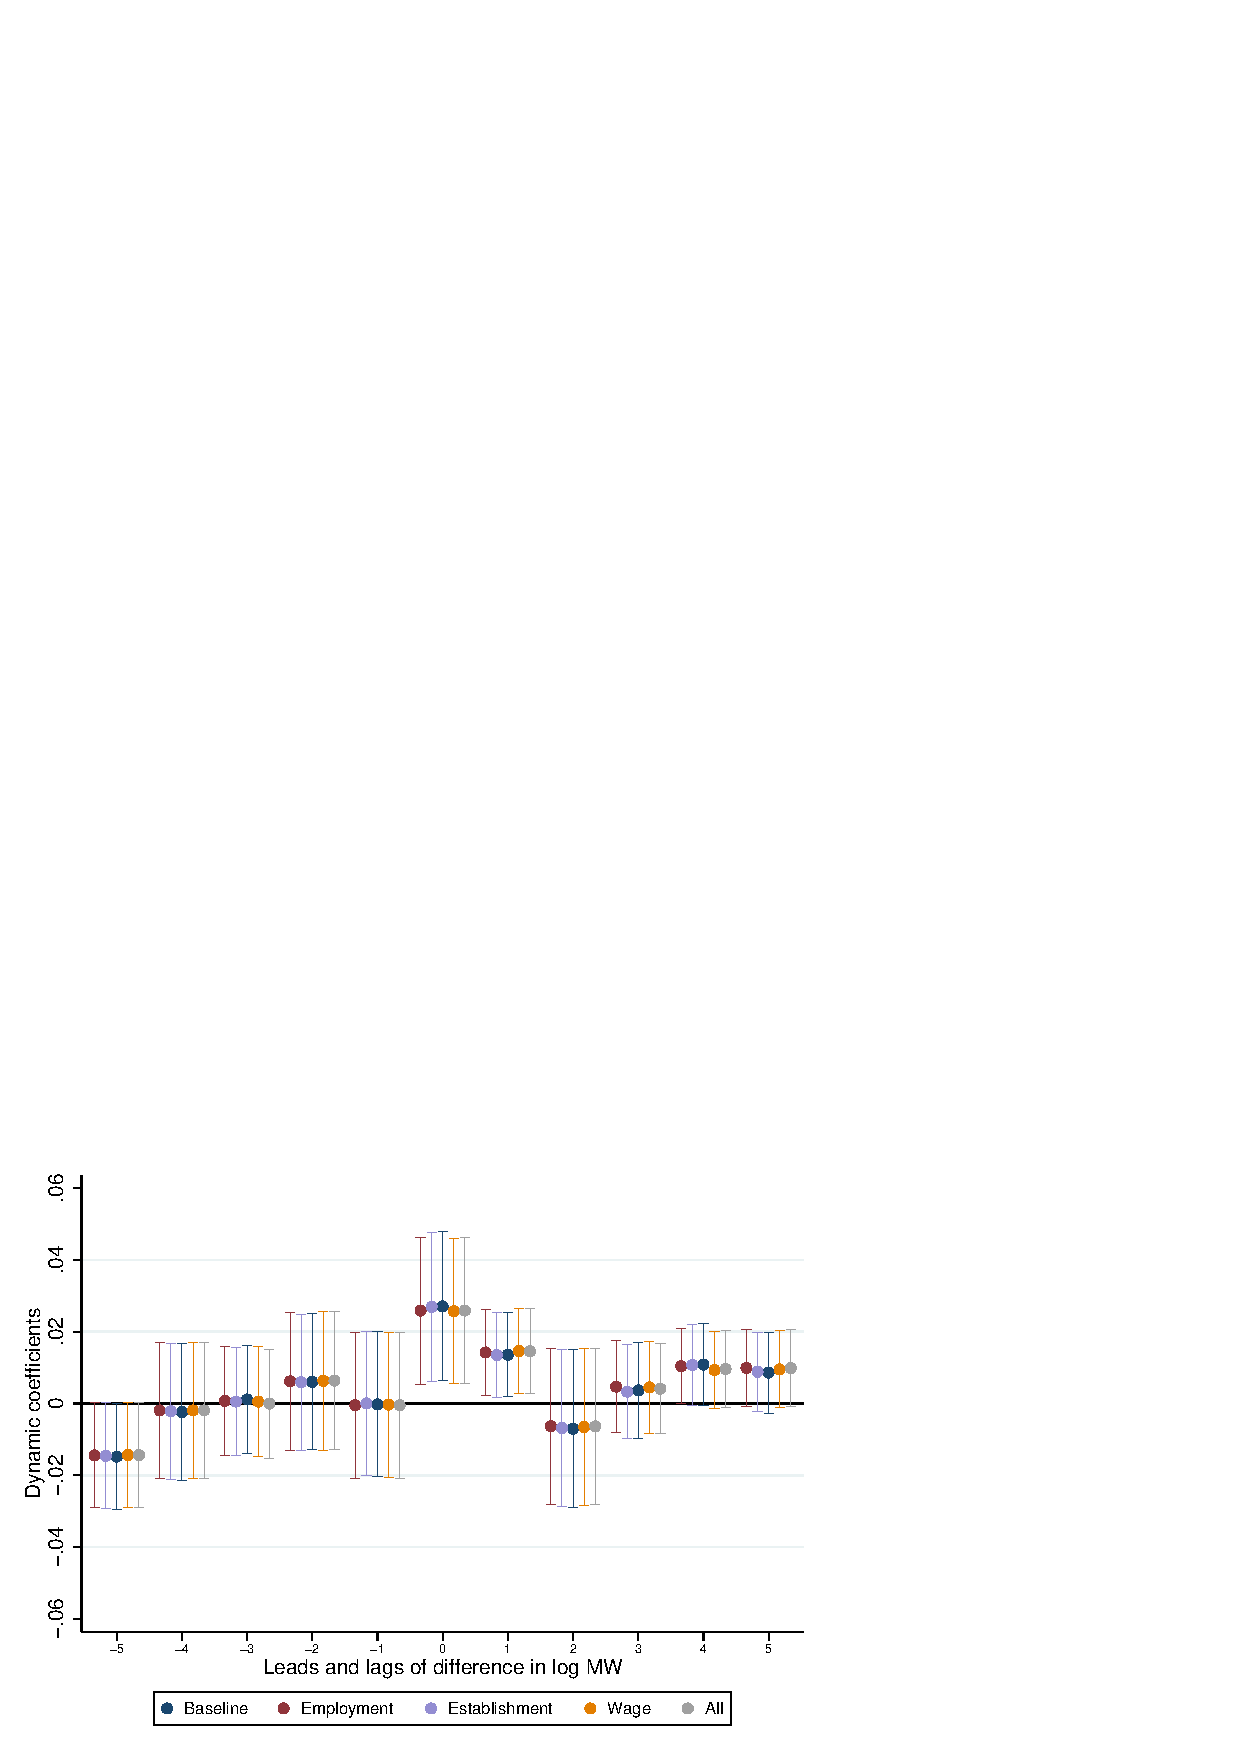
\includegraphics[width = 0.7\textwidth]{../../analysis/first_differences/output/fd_models_control.png}
	\begin{minipage}{.95\textwidth} \footnotesize
		\vspace{2mm} 
		\textit{Notes}: The figure show estimates for $\hat{\beta}_{r}$ obtained from 
		\autoref{eq:leads_lags} when progressively adding time-varying controls for local shocks. 
		The \textit{baseline} series plots coefficients taken from 
		\autoref{tab:dynamic_leads_lags_econshock}, column (1). The \textit{employment}, 
		\textit{establishment}, \textit{wage}, and \textit{building} series plot coefficients 
		from \autoref{tab:dynamic_leads_lags_econshock}, columns (2) to (5) respectively. 90 
		percent confidence intervals reported.  
	\end{minipage}
\end{figure}

\clearpage
%%%%%%%%%%%%%%%%%%%%%%%%%%%%%%%%%%%%%%%%%%%%%%%%%%%%%%%%%%%%%%%%%%%%%%%%%%%%%%%%%
\section{A toy model of the local housing market}\label{sec:model}

We build a simple model that is used to build a benchmark estimate of the effect of MW
policies on rents.

\subsection{Model set-up}

We focus on the supply and demand of housing in a given zipcode. Consider an environment with 
an exogenously given continuum of households in each zipcode divided in two groups: minimum wage 
and non-minimum wage households (HH). The former are fully affected by the MW, whereas the latter 
are not affected at all.

On the supply side, we denote by $H$ the continuous measure of housing units available for rent 
in the zipcode. We assume that units are homogeneous, and can be rented at the a rent of $r$. The 
supply of housing $H(r)$ is assumed to be increasing in rents $r$, so that $H'(r) > 0$.

Let us move to the demand side. Households receive monthly a income, which we denote by 
$\underline{w}$ and $w$ for MW HH and non-MW households, respectively. Demand for housing is given 
by $\underline{H}(r, \underline{w})$ and $\overline{H}(r, w)$ for each household type. We make two 
standard assumptions on these objects: (i) the demand of housing is downward sloping (i.e., 
$\underline{H}_r(r, \underline{w}) < 0$ and $\overline{H}_r(r, w) < 0$); and (ii) the demand for 
housing is increasing in income (i.e., $\underline{H}_w(r, \underline{w}) > 0$ and $\overline{H}_w(r, 
w) > 0$)


\subsection{Equilibrium and the elasticity of rents to the minimum wage}

Equilibrium rents $r^*$ are such that local housing supply is equated to local housing demand. 
Formally,

\begin{equation*}\label{eq:model-eq}
H(r) =  \underline{H}(r, \underline{w}) + \overline{H}(r, w) \ .
\end{equation*}

We are interested in the elasticity of equilibrium rents $r^*$ to the minimum wage $\underline{w}$, 
which we denote by $\rho$. The implicit function theorem applied on the above equation yields

\begin{equation}\label{eq:model-elasticity}
\rho := \frac{d \ln r^*}{d \ln \underline{w}} 
= \frac{\underline{w} \ \underline{H}_w}
{r\  H'(r) - r \ \underline{H}_r - r \ \overline{H}_r} \ ,
\end{equation}
where we denote partial derivatives with sub-indexes.

Note that, since $\underline{H}_r < 0$ and $\overline{H}_r < 0$, the above expression is always 
positive. When the MW increases the local housing market moves to a new equilibrium with higher 
rents. The magnitude of the elasticity is driven by the relative magnitudes of the earnings of 
minimum wage workers ($\overline{w}$) and rents ($r$), and the slopes of the different 
functions in equilibrium. For instance, a higher response of housing demand to the minimum wage 
change ($\underline{H}_w$) would result in a higher elasticity.